\section{Introduction to Aeronautics}
Since, we assume that reader may not necessarily have Aeronautics/ Mechanical background, we will try to introduce to some basic concepts required to follow subsequent sections. For a detailed introduction, we recommend excellent texts\cite{anderson2005introduction}, \cite{anderson1999aircraft}.

Let us look at the simplest case of level unaccelerated flight. Drawing similarity from ground body.
TODO: insert figure
In order to balance all forces, we need to oppose gravity and oppose aerodynamic drag similar to friction in ground bodies. Force opposing gravity ie. weight($F_g$) is called lift($F_L$) and drag($F_D$) is compensated by generated thrust($F_T$).

Now, let us take case of earliest flying body we have seen ie. paper planes. To study aerodynamic forces a paper palne, we can assume flat plate theory\cite{tangler2005wind}.
\begin{align}
    \begin{split}
        \nonumber
        F_a &: \text{aerodynamic force} \\
        &= \frac{dp}{dt} = \frac{dm}{dt} v_n  \\
        &= v_n \frac{\rho A dx}{dt} = v_n (\rho A v_\infty) \\
        &= \rho A v_\infty^2 \sin(\theta) \\
    \end{split}\\
        \label{eq:flat_lift}
        F_L &= F_a \cos(\theta) = \rho A v_\infty^2 \sin(\theta) \cos(\theta)\\
        \label{eq:flat_drag}
        F_D &= F_a \sin(\theta) = \rho A v_\infty^2 \sin^2(\theta)\\        
    \begin{split}
        \nonumber
        \text{Here},\\
        v_\infty &: airspeed\\
        v_n&: \text{speed normal to surface}\\
        p&:\text{air momentum}\\
        A&:\text{area of plate}\\
        \theta&:\text{angle of attack}\\    
    \end{split}
\end{align}

\begin{align*}
%\label{eq:flat_drag}\\
\end{align*}

Note, even though this model makes too many oversimplifying assumptions(imcompressible, always seperated flow), it works surprisingly well to model\cite{cory2008experiments} and perch flat plate glider on wire\cite{moore2014robust}. The glider experiences angle of attack as high as 90\textdegree - 120\textdegree which are well beyond in stall regime(angle at which flow becomes seperated), yet data fits nicely with additional gaussian radial basis function.

In practice though, we always use aerofoil shape over flat plate since aerofoil shape keeps flow attached(laminar) at higher angles and gives higher lift to drag ratio. Lift and drag for wing by lifting line theory is modelled as:
\begin{align}
    \label{eq:airfoil}
    \begin{split}
        F_L &= q_\infty S C_l \\
        F_D &= q_\infty S C_d \\
        \text{where,}\\
        q_\infty &\doteq \frac{\rho v_\infty^2}{2} \\
        C_l &: \text{lift coeffecient}\\
        &\doteq C_l(\alpha, v_\infty, \text{Re})\\
        C_d &: \text{drag coeffecient}\\
        &= C_{d0} + \frac{C_l^2}{\pi e AR}\\
        \alpha&:\text{angle of attack}\\
        n_\text{Re}&: \text{Reynolds number}\\
        C_{d0} &: \text{parasitic drag} \\
        e &: \text{oswald effeciency factor} \\
        AR &: \text{aspect ratio of wing}
    \end{split}
\end{align}
TODO: insert plot for cl , cd vs alpha

Drag forces, are always produced as byproduct of lift as can be seen from \eqref{eq:flat_lift} and \eqref{eq:flat_drag}. This drag is called (lift)\textbf{induced drag}, while drag due to skin friction is called \textbf{parasitic drag}.Now that we know how to balance vetical forces ie. gravity $F_g$ with lift $F_L$, lets see how to generate thrust $F_T$ to oppose drag force $F_D$. Thrust is generated by propulsion sytems:
\begin{itemize}
\item Jet propulsion
\item Rotory propeller
\end{itemize}
Immediately question aries, which one is more effecient? From Newtons's second law, rate of momentum change gives force $T$ (eq. 3.1 \cite{anderson1999aircraft}):
\begin{align*}
    T&=\dot{m}(v_e - v_\infty)\\
    \dot{m}&:\text{mass flow}\\
    v_e&: \text{exit speed of air}\\
\end{align*}
Since, kinetic energy imparted air, is wasted once exited. This gives an intution about effeciency that moving large mass to small speeds(rotory propeller) is more effecient over moving small mass to large speed. But there is a thrust effeciency tradeoff. Formally, effeciency($\eta_p$) is given by(eq. 3.8 \cite{anderson1999aircraft}).
 \begin{equation*}
     \eta_p = \frac{2}{1+v_e/v_\infty}
 \end{equation*}

So back to our question, which to use? This depends on speed for which vehicle is designed to fly. At low speeds rotory propellers are more effecient but effeiency decreases with increasing airspeed while jet propulsion effeciency is constant w.r.t airspeed and is hence more effecient at high speed.

\subsection{Propellers}
We can think propeller to be nothing but just a rotating wing. Since wings generate lift at high airspeeds, this relative speed is generated by instead rotating propellers at high speed. We can model $F_{prop}$ by integrating $F_l$ and $F_d$ of each section over blade length. This method is known as Blade Element Theory(BET). But for sake of simplicity, we will use momentum theory \cite{momentum_prop}.
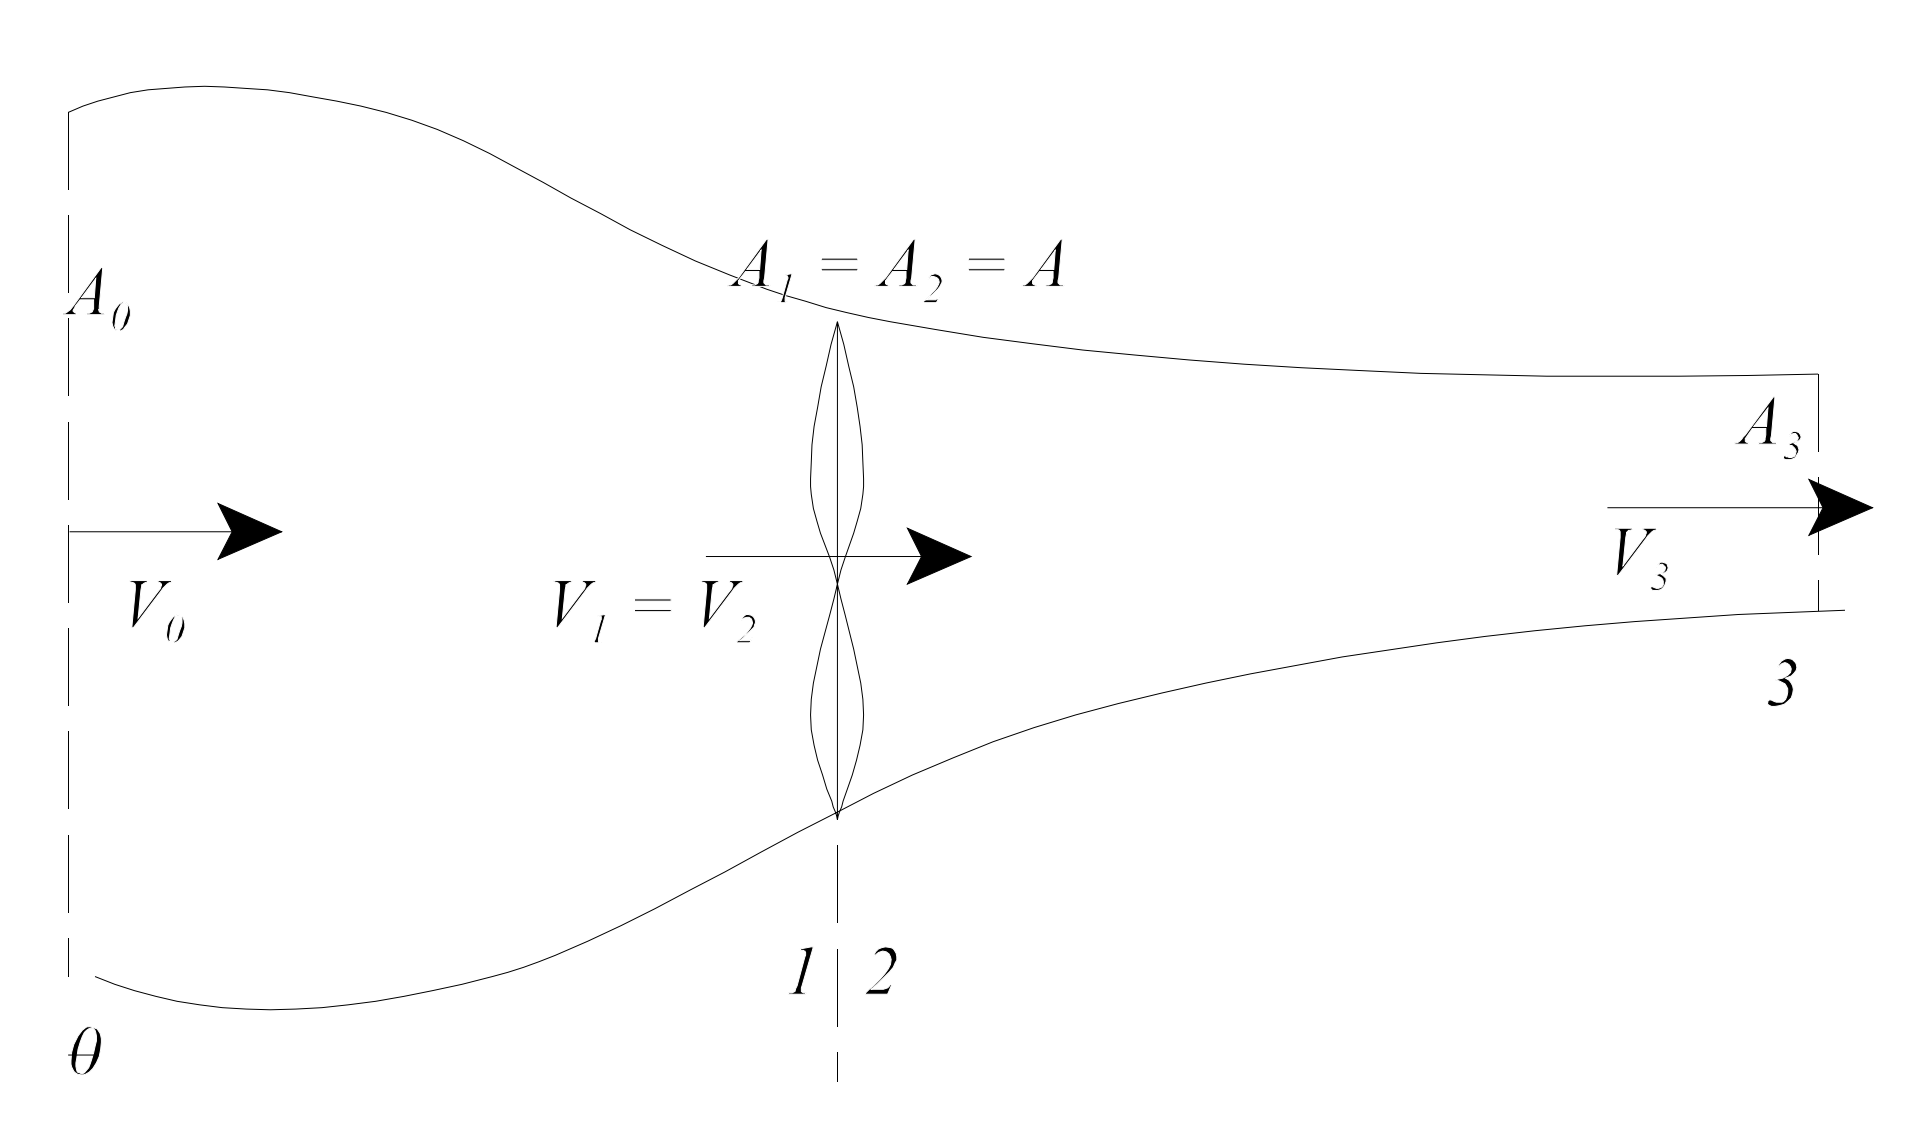
\includegraphics[width=\textwidth]{prop_momentum}
Applying Bernoulli’s equation:
\begin{align}
    \label{one}
    P_\infty + \frac{1}{2}\rho v_0^2 &= P_1 + \frac{1}{2}\rho v_1^2 \\
    \label{two}
    P_\infty + \frac{1}{2}\rho v_3^2 &= P_2 + \frac{1}{2}\rho v_2^2
\end{align}
deducting \eqref{two} from \eqref{one} and note $v_1=v_2$,
\begin{equation}
    \label{eq:p_delta}
    P_2 - P_1 = \frac{1}{2}\rho(v_3^2 - v_0^2)
\end{equation}
Thrust by momentum change and pressure difference across propeller times area swept gives:
\begin{align}
    \label{eq:three}
    T &= \rho A_3 v_3(v_3-v_0)\\
    \label{eq:four}
    T &= A(P_2 - P_1)
\end{align}
By mass conservation, $Av_1 = A3v_3$ in \eqref{eq:three}. equating \eqref{eq:three} and \eqref{eq:four} and together with \eqref{eq:p_delta} gives:
\begin{equation}
    \label{eq:v_avg}
    v_1 = \frac{v_0+v_3}{2}
\end{equation} 
\eqref{eq:v_avg} states that speed through propeller is average of entry and exit. Overall momentum theory gives thrust(complete proof ref. to \cite{momentum_prop}):

\begin{align}
    \label{eq:thrust_momentum}
    T &= P_i^{2/3} (2 \rho A)^{1/3}\\
    \nonumber
    P_i &: \text{Induced power (engine power)}
\end{align}

Now, that we have some rudimentary understanding of theory, we can begin with UAV design in next section.